\chapter{Constrained Clustering}\label{ch:ConstrainedClustering}

Once the basics concepts about clustering have been introduced, we can focus on defining the concepts specific to constrained clustering. We give example applications and highlight its advantages and disadvantages. To this end we take as our main reference the survey presented in \cite{davidson2007survey}. We describe the motivation for constrained clustering in Section \ref{sec:CCMotiv}. We formalize the concept of constraints and discuss their use in Sections \ref{sec:ConstDef} and \ref{sec:ConstUse} respectively. Afterwards a list of applications of constrained clustering is presented in Section \ref{sec:CCApplications}. Benefits and problems, as well as solutions for these problems, are discussed in Sections \ref{sec:ConstraintsBenefits} and \ref{sec:ConstraintsProblems} respectively.

\section{Motivation for Constrained Clustering} \label{sec:CCMotiv}

As we discussed in Chapter \ref{ch:IntroClustering}, unsupervised clustering methods are useful for structuring data referring to a particular area. An example of this can be found in text classification; In \cite{cohn2003semi} a problem proposed by Yahoo! is addressed. The problem consists in, given a large number of text documents, grouping them according to a taxonomy in which documents with similar topics are conceptually nearby. To solve this problem, unsupervised clustering methods are useful, as there is limited initially available information on the problem. However, in \cite{wagstaff2001constrained} it is shown that applying unsupervised clustering to certain problems, such as grouping \acf{GPS} data in such a way that clusters define the lanes of a road, does not produce significant results, as the clusters obtained are far from the elongated shape that would be expected. To tackle the problem, they introduced a new element in clustering, the \textit{constraint}, which made it possible to include domain knowledge to guide clustering methods towards the expected results. It was enough to indicate that the lanes of the road on which the vehicles circulate are four meters wide, and therefore any vehicle that is at a distance of more than 4 meters from another, perpendicular to the motion direction, must be located in a different cluster.

We are now in a new scenario: it is possible to incorporate additional information into the clustering process, in addition to that contained in the dataset itself, to guide it in the formation of the output partition and obtain more accurate results. This new approach is known as constrained clustering, an \acf{SSL} paradigm, unlike traditional clustering methods which fall into the category of unsupervised learning. 

\section{Constraints Definition} \label{sec:ConstDef}

The new type of information that we incorporate into clustering is given in the form of instance-level constraints. Their purpose is to specify whether two instances ($x_i$ and $x_j$) from the dataset ($X$) must be in the same cluster or, on the contrary, they must be in separate clusters.

Constraints that indicate that two instances must be placed in the same cluster are called \acf{ML}, and are noted with $C_=(x_i,x_j)$. Similarly, constraints that specify that two instances must not be placed in the same cluster are called \acf{CL}, and are noted with $C_{\neq}(x_i,x_j)$ \cite{wagstaff2000clustering}.

Although they may seem simple, constraints defined as above have some very interesting properties. \acs{ML} constraints are an example of an equivalence relation, and therefore are symmetrical, reflexive and transitive. Observation \ref{ob:MLConstraintsRelation} formalizes this concept. On the other hand, and although \acs{CL} do not constitute an equivalence relation, they feature other properties, formalized in Observation \ref{ob:CLConstraintsRelation}.

\begin{observation}
	\textbf{Must-link constraints are transitive.} Let $CC_i$ and $CC_j$ be connected components (completely connected subgraphs by \acs{ML} constraints), and let $x_i$ and $x_j$ be the instances in $CC_i$ and $CC_j$ respectively. Then $C_=(x_i,x_j): x_i \in CC_i, x_j \in CC_j \rightarrow C_=(x_a,x_b) \forall x_a, x_b: x_a\in CC_i, x_b \in CC_j$ \cite{davidson2007survey}.
	\label{ob:MLConstraintsRelation}
\end{observation}

\begin{observation}
	\textbf{Cannot-link constraints can be entailed.} Let $CC_i$ and $CC_j$ be connected components (completely connected subgraphs by \acs{CL} constraints) and let $x_i$ and $x_j$ be the instances in $CC_i$ and $CC_j$ respectively. Then $C_{\neq}(x_i, x_j): x_i \in CC_i, x_j \in CC_j \rightarrow _{\neq}(x_a, x_b) \forall x_a, x_b: x_a\in CC_i, x_b \in CC_j$ \cite{davidson2007survey}
	\label{ob:CLConstraintsRelation}.
\end{observation}

A clear example of the use of constraints can be found in clustering applications where there are distance measurement limitations, as in the case of \acs{GPS} data. Thus, if we want instances forming two clusters to be separated by a distance greater or equal to $\delta$, it is enough to set \acs{ML} constraints between all instances separated by less than $\delta$ units. Similarly, if we want the diameter of the clusters to be at most $\epsilon$, we must set \acs{CL} constraint between instances separated by more than $\epsilon$ units. Figure \ref{fig:DistanceConstraints} shows a graphical representation of these two types of constraints.

\begin{figure}[!h]
	\centering
	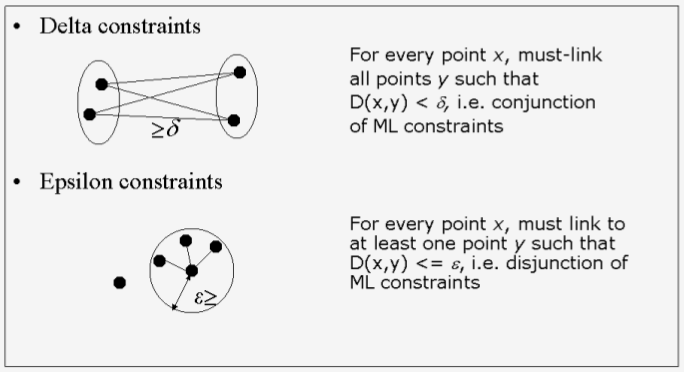
\includegraphics[scale=0.45]{gfx/ConstClust/RestriccionesDeltaEpsilon.png} 
	\caption[\textit{delta} $(\delta)$ and \textit{epsilon} $(\epsilon)$ constraints.]{\textit{delta} $(\delta)$ and \textit{epsilon} $(\epsilon)$ constraints \cite{davidson2007survey}.}\label{fig:DistanceConstraints}
\end{figure}


\section{Use of Constraints} \label{sec:ConstUse}

While supervised learning involves knowing the label associated with each instance, \acs{SSL} has only a subset of labeled instances. On the other hand, in many domains the available information refers to relations between instances, and not to the specific class to which they belong. Moreover, in interactive clustering systems, a user who is not expert in the problem domain will probably be able to provide information in the form of constraints such as \acs{ML} and \acs{CL}, instead of providing information on what particular class certain instances belong to \cite{cohn2003semi,davidson2007hierarchical}.

Typically, constraints are incorporated into clustering problems in two ways. They can be used to alter the rules of assignment of instances to clusters of the method in question, so that the solution satisfies as many constraints as possible. Alternatively, it is possible to train the distance function used by the method based on the constraints, either before or during the application of the method. In any case, the initialization phase can take the constraints into account, so that instances appearing together in \acs{ML} constraints will be placed in the same cluster, and those between which there is a \acs{CL} constraint will be placed in different clusters. Based on this distinction, we identify two ways of approaching the problem: those based on explicit constraints (\textit{constraints-based}) and those based on distances (\textit{distance-based}).

\subsection{Constraints-based Methods}

In constraints-based methods, the clustering method itself is modified in such a way that the available information is used to bias the search and obtain an appropriate data partition.

Regarding the degree to which the constraints have to be satisfied, we can make a distinction between the concepts of hard \cite{wagstaff2001constrained,davidson2005agglomerative} and soft \cite{law2004clustering,basu2004active,segal2003discovering,davidson2005clustering,law2005model} constraints. Hard constraints must necessarily be satisfied in the output partition of any algorithm that makes use of them, while soft constraints are taken as a strong guide for the algorithm that uses them but can be partially satisfied in the output partition \cite{seret2014new}. For the purposes of this work, we will employ the latter. There are several techniques to obtain a partition based on constraints:

\begin{itemize}
	
	\item Modifying the objective function to include a penalty term for breaking constraints \cite{demiriz1999semi,davidson2005clustering}.
	
	\item Grouping instances with additional information obtained from a conditional distribution into an auxiliary space \cite{sinkkonen2000semisupervised}.
	
	\item Enforcing all constraints to be satisfied by modifying the the instance clusters assignment rule \cite{wagstaff2001constrained}.
	
	\item Initializing clusters based on constraints inferred from a set of labeled instances \cite{basu2002semi}.
	
\end{itemize}

Figure \ref{fig:ConstClustOverDataset} shows a dataset together with its associated constraints and proposes a possible clustering that satisfies all constraints.

\begin{figure}[bth]
	\myfloatalign
	\subfloat[Constraints over a dataset.]
	{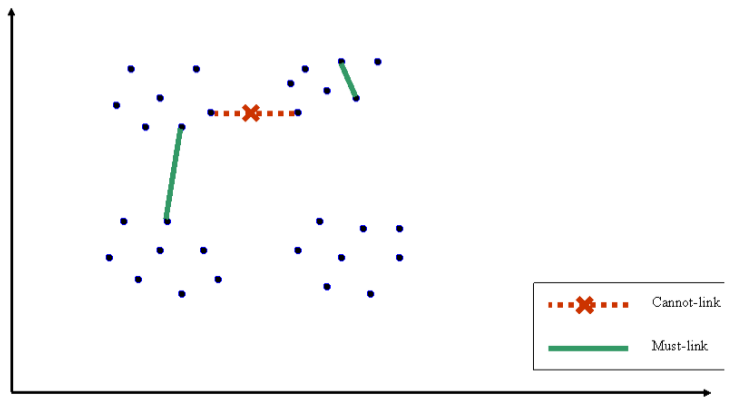
\includegraphics[width=.45\linewidth]{gfx/ConstClust/InputInstancesAndConst1}}
	\hspace{1cm}
	\subfloat[Clustering satisfying all constraints.]
	{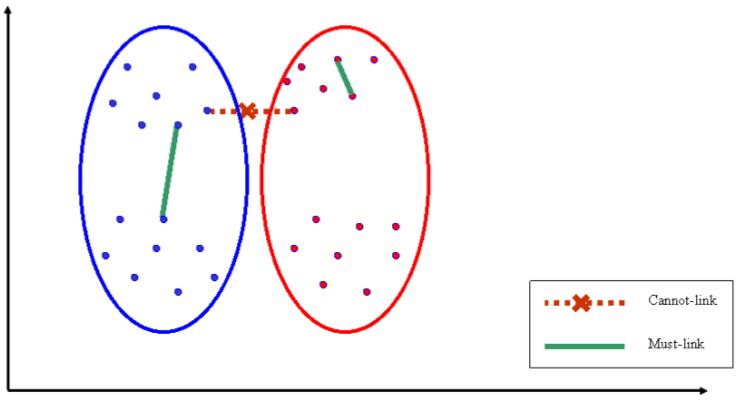
\includegraphics[width=.45\linewidth]{gfx/ConstClust/ClusteringSatAll}}
	
	\caption[Constraints and clustering over a dataset.]{Constraints and clustering over a dataset \cite{davidson2007survey}.} \label{fig:ConstClustOverDataset}
\end{figure}

\subsection{Distance-based Methods}

In distance-based approaches, classic clustering methods that use a distance measurement are modified so that the distance measurement incorporates the constraints. In this context, constraint satisfaction means that instances co-occurring in \acs{ML} constraints are placed together in the space, and those co-occurring in \acs{CL} are separated.

Figure \ref{fig:ConstrainsAndMetricLearned} shows a possible clustering based on a metric learned from the constraints. It should be noted that in Figure \ref{fig:MetricLearned} the data space has been compressed on the vertical axis and expanded on the horizontal axis to match the learned distance metric.

\begin{figure}[bth]
	\myfloatalign
	\subfloat[Constraints over a dataset.]
	{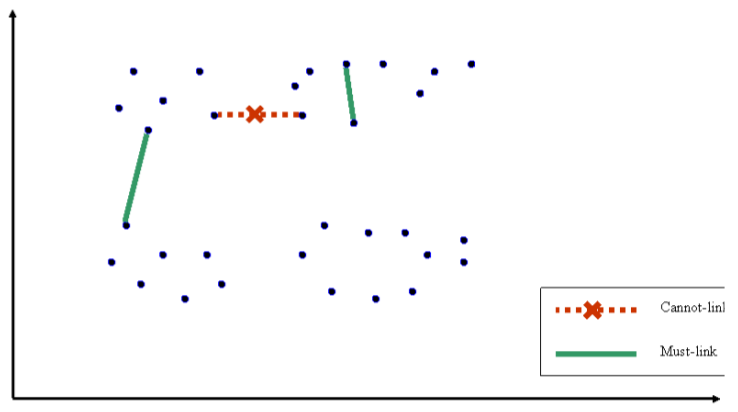
\includegraphics[width=.45\linewidth]{gfx/ConstClust/InputInstancesAndConst2}} 
	\hspace{0.5cm}
	\subfloat[Clustering based on a metric learned from constraints.]
	{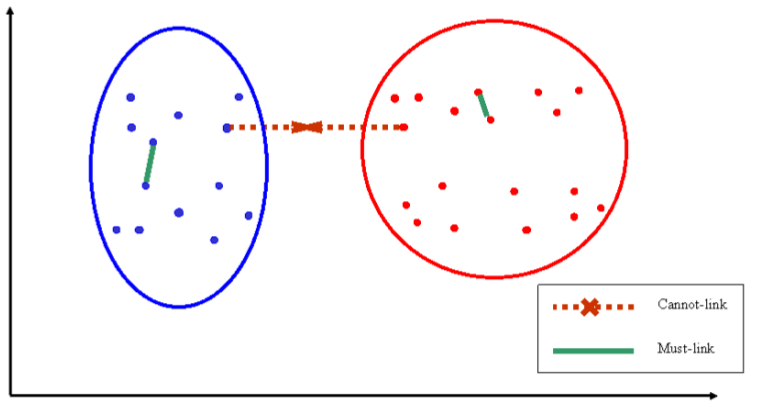
\includegraphics[width=.45\linewidth]{gfx/ConstClust/MetricaAprendida}
	\label{fig:MetricLearned}}
	\caption[Clustering based on a metric learned from constraints.]{Clustering based on a metric learned from constraints \cite{davidson2007survey}.} \label{fig:ConstrainsAndMetricLearned}
\end{figure}

\section{Constrained Clustering Applications} \label{sec:CCApplications}

This section shows some application cases in which constrained clustering has turned out to be a more useful tool than fully unsupervised clustering. For each case we will analyze how the constraints were obtained and how they improve the resulting clustering. 

\subsection{Image Analysis}

Figure \ref{fig:CMUFacesDatabase} shows a sample from the \acsfont{CMU} (Carnegie Mellon University) faces dataset, where the task is to group faces according to different criteria (in this case, face orientation).

\begin{figure}[bth]
	\myfloatalign
	\subfloat[Profile faces.]
	{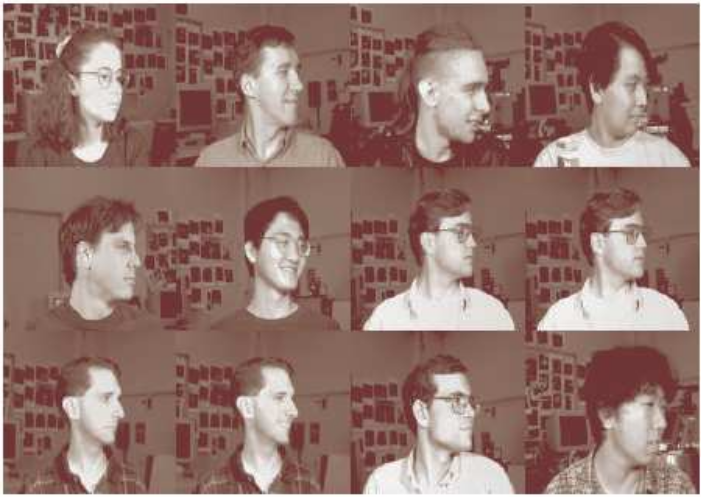
\includegraphics[width=.3\linewidth]{gfx/ConstClust/AnalisisImagenes/Caras1}} \quad
	\subfloat[Front faces.]
	{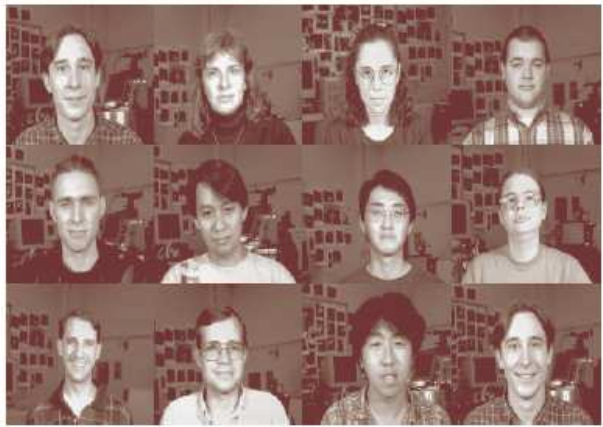
\includegraphics[width=.3\linewidth]{gfx/ConstClust/AnalisisImagenes/Caras3}} \quad
	\subfloat[Faces up.]
	{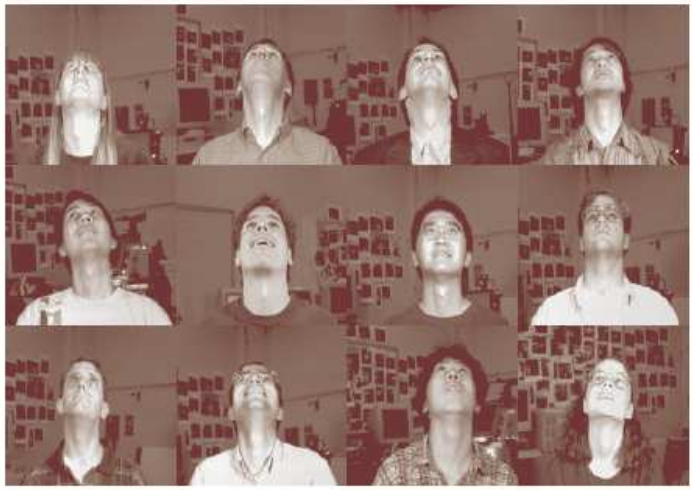
\includegraphics[width=.3\linewidth]{gfx/ConstClust/AnalisisImagenes/Caras2}} \quad
	\caption[\acsfont{CMU} faces database.]{\acsfont{CMU} faces database \cite{davidson2007survey}.}\label{fig:CMUFacesDatabase}
\end{figure}

The method used to obtain the constraints is one of the most popular in the literature: let the number of clusters of the resulting partition be equal to the number of classes in the database, and generate the constraints from a subset of labeled instances; in other words, if two instances have different labels, set a \acs{CL} constraint between them, and otherwise set an \acs{ML} one. Thus, between the images shown in Figure \ref{fig:FacesDatabaseCL} \acs{CL} constraints are set, since, although they depict the same person, they do not have the same orientation.

\begin{figure}[bth]
	\myfloatalign
	{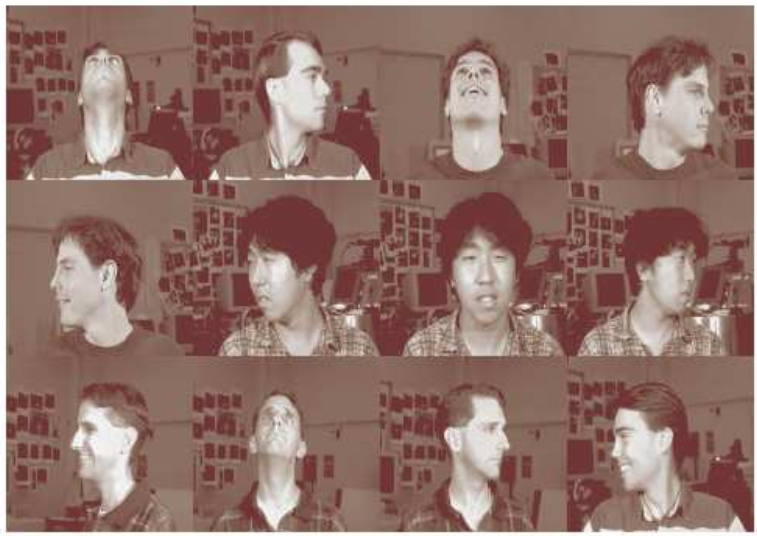
\includegraphics[width=.35\linewidth]{gfx/ConstClust/AnalisisImagenes/CarasDifOr1}} \quad
	{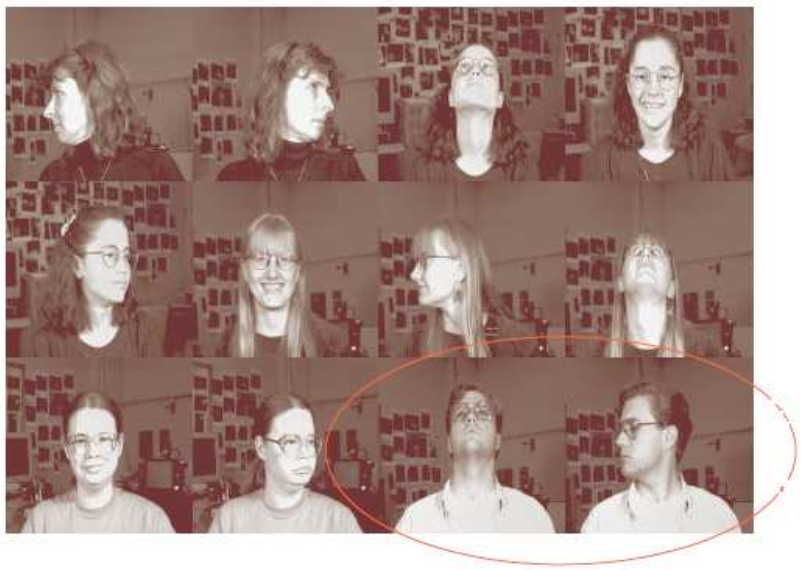
\includegraphics[width=.35\linewidth]{gfx/ConstClust/AnalisisImagenes/CarasDifOr2}}
	\caption[\acs{CL} constraints between faces of the same person.]{\acs{CL} constraints between faces of the same person \cite{davidson2007survey}.}\label{fig:FacesDatabaseCL}
\end{figure}

Figure \ref{fig:AiboRobotClustSys} shows another set of image data to which constrained clustering techniques are applied. In this case, the task is to perform object recognition to incorporate the method into the navigation system of the Aibo robot \cite{davidson2005clustering}. Distance constraints such as $\delta$ and $\epsilon$ are used as described in Figure \ref{fig:DistanceConstraints}. In this way, well differentiated clusters are obtained and therefore they are useful for the path-finding tasks performed by the robot during navigation.

\begin{figure}[bth]
	\myfloatalign
	\subfloat[Original image.]
	{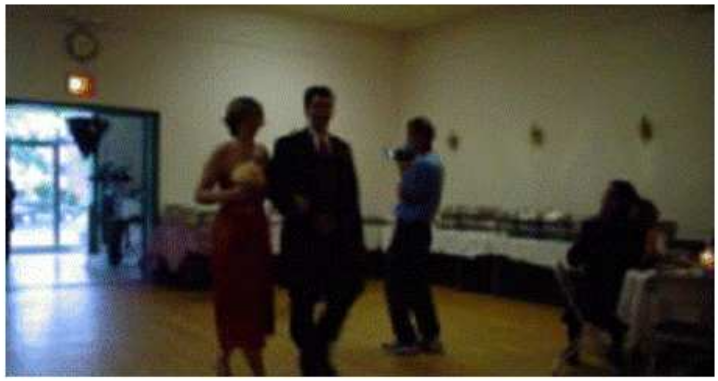
\includegraphics[width=.3\linewidth]{gfx/ConstClust/AnalisisImagenes/Aibo1}} \quad
	\subfloat[Classic clustering.]
	{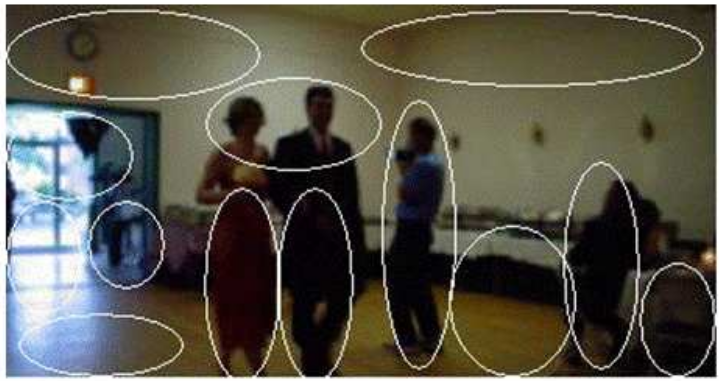
\includegraphics[width=.3\linewidth]{gfx/ConstClust/AnalisisImagenes/Aibo2}} \quad
	\subfloat[Constrained clustering.]
	{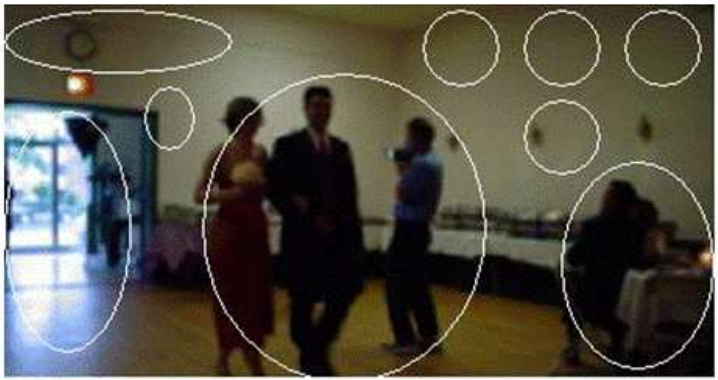
\includegraphics[width=.3\linewidth]{gfx/ConstClust/AnalisisImagenes/Aibo3}} \quad
	\caption[Clustering method used in Aibo robot navigation system.]{Clustering method used in Aibo robot navigation system \cite{davidson2007survey,davidson2005clustering}.}\label{fig:AiboRobotClustSys}
\end{figure}

\subsection{Video Analysis}

Video databases are one example where constraints can be generated directly from the data domain, especially if space-time metadata is available \cite{yan2006discriminative}. In time-sequenced data it is possible to set \acs{ML} constraints between groups of pixels of frames close in time. This is especially useful when the task is to perform object recognition based on clustering and segmentation. It is also possible to add \acs{CL} constraints to image segments in the same snapshot, as the probability of them being associated with the same object after segmentation is low. In fact, in video analysis problems there are a variety of constraint extraction methods \cite{yan2006discriminative}. Figure \ref{fig:ConstExtractionVideo} shows some examples. 

\begin{figure}[bth]
	\myfloatalign
	\subfloat[]
	{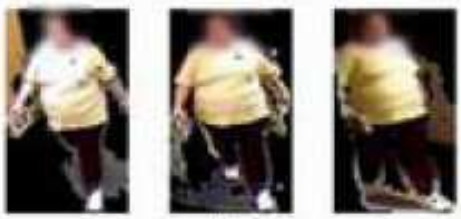
\includegraphics[width=.4\linewidth]{gfx/ConstClust/Videos/VideoA}
	\label{fig:ConstExtractionVideoA}}
	\quad
	\subfloat[]
	{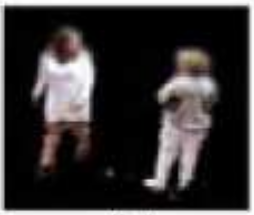
\includegraphics[width=.225\linewidth]{gfx/ConstClust/Videos/VideoB}
	\label{fig:ConstExtractionVideoB}} \quad
	\subfloat[]
	{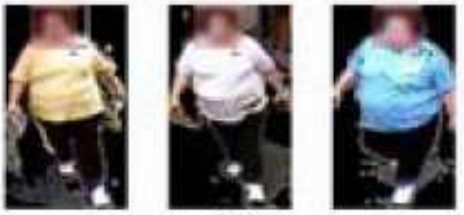
\includegraphics[width=.4\linewidth]{gfx/ConstClust/Videos/VideoC}
	\label{fig:ConstExtractionVideoC}}
	\quad
	\subfloat[]
	{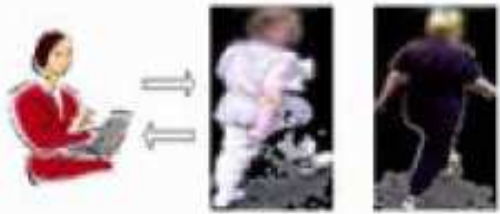
\includegraphics[width=.4\linewidth]{gfx/ConstClust/Videos/VideoD}
	\label{fig:ConstExtractionVideoD}}
	\caption[Constraints extraction in video data.]{Constraints extraction in video data \cite{yan2006discriminative,davidson2007survey}.}\label{fig:ConstExtractionVideo}
\end{figure}

In Figure \ref{fig:ConstExtractionVideo}, image \ref{fig:ConstExtractionVideoA} corresponds to constraints extracted from tracking a person over a period of time; \ref{fig:ConstExtractionVideoB} corresponds to spatial constraints associating two objects located in the same frame; image \ref{fig:ConstExtractionVideoC} corresponds to constraints obtained through facial recognition, and \ref{fig:ConstExtractionVideoD} to those provided by the user.

With so many constraint extraction methods, one might ask: What happens if too many constraints are imposed? Does this make the problem over-constrained? In Section \ref{sec:ConstraintsProblems} we will address these questions.

\subsection{Biological Data}

In gene clustering based on microarray data, genes are represented by their expression profile in different experiments and grouped using different constrained clustering methods. Figure \ref{fig:GeneticApp} shows an example: these are \acs{ML} constraints set between genes based on co-occurrence data stored in the protein interaction database, which contains information about which genes---and their associated proteins---are present in the same cell processes \cite{xenarios2001dip}. This information can be used to improve results provided by clustering methods. \cite{segal2003discovering}.

\begin{figure}[!h]
	\centering
	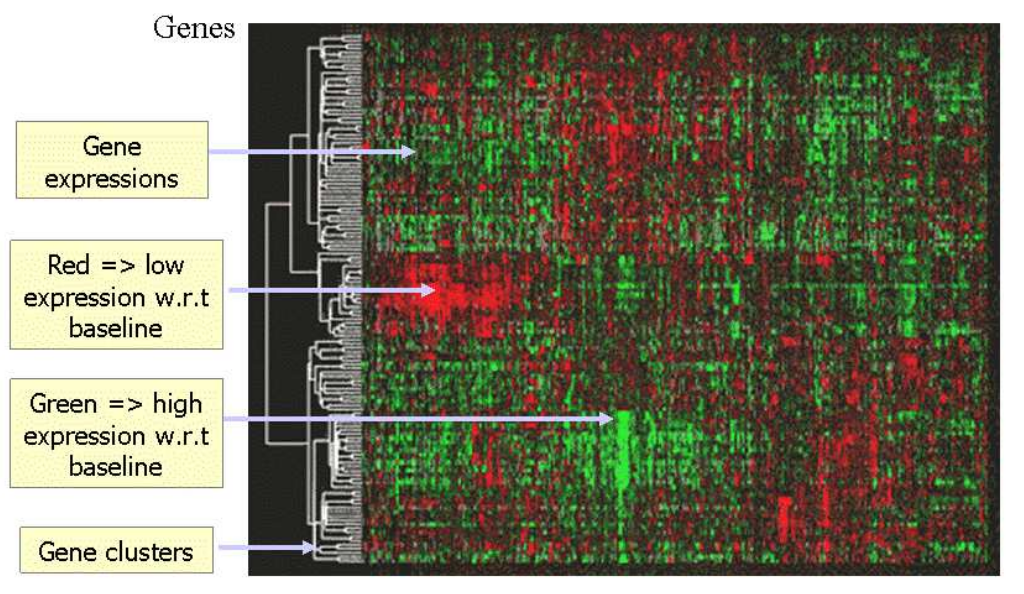
\includegraphics[scale=0.3]{gfx/ConstClust/Genetica/Genes} 
	\caption[Gene clustering based on microarray data.]{Gene clustering based on microarray data \cite{davidson2007survey}.}\label{fig:GeneticApp}
\end{figure}

\subsection{Text Analysis}

In content classification tasks, the goal is to automatically split large amounts of documents into groups or clusters. In this case it is possible to extract constraints from multiple auxiliary resources. For example, if two documents are in the same directory, an \acs{ML} constraint could be set between them. This way, it is possible to adjust the resulting clustering to suit a particular criterion, such as creating a hierarchy of documents akin to the way they are organized in the original directory structure.

\subsection{Web Data} 

Constrained clustering is very useful in web search data processing. Here, the aim is to automatically group the results of an ambiguous query to the search engine into clusters of \acsp{URL}, which represent the queried concept in different contexts. In this area it is possible to extract the constraints from previous searches performed by other users, so that an \acs{ML} constraint is set between \acsp{URL} visited in the same user session. Clustering using these constraints can help bias search results towards user preferences.

\subsection{Audio Data}

In certain audio analysis tasks, the number of object classes present in the data may not be known, although constraints can be extracted directly from the data domain. This happens, for example, when applying clustering to speaker recognition in a conversation \cite{bar2003learning}. In this case the number of participants is not known a priori, but it is easy to detect if two speakers are different or similar and to set constraints accordingly.

\subsection[\acsfont{GPS} Data]{GPS Data} \label{sec:GPSApp}

As mentioned at the beginning of Chapter \ref{ch:ConstrainedClustering}, constrained clustering can be applied to \acs{GPS} data in order to identify the lane each vehicle is in, as shown in Figure \ref{fig:GPSClustData}. Each instance is represented by the position it occupies on the road in two-dimensional Cartesian coordinates $(x,y)$ obtained from \acs{GPS} data. Figure \ref{fig:figure15} graphically shows this representation of the data. Note that multiple instances can refer to the same vehicle at different times.

\begin{figure}[!h]
	\centering
	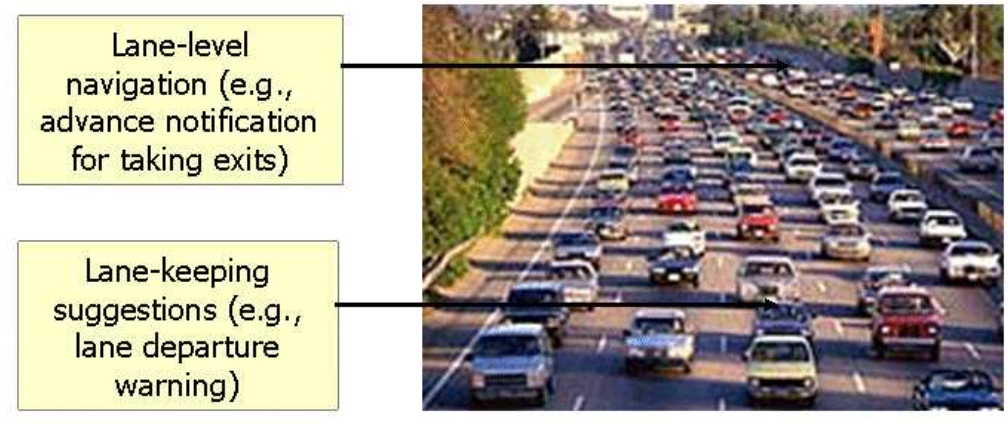
\includegraphics[scale=0.3]{gfx/ConstClust/GPS/Coches} 
	\caption[\acs{GPS} data use.]{\acs{GPS} data use \cite{davidson2007survey, wagstaff2001constrained}.}\label{fig:GPSClustData}
\end{figure}

In this domain, real clusters have an elongated shape on the horizontal axis and are aligned perpendicularly to the motion direction. To produce clusters with this shape, we can make use of constraints. We will set \acs{CL} constraints between those instances more than four meters apart perpendicularly to the motion direction---since the lanes have a maximum width of four meters---and \acs{ML} constraints between those instances that present continuity in the motion direction axis, since it is likely that the vehicles they represent are in the same lane. This clustering model has proven to be very useful in real-time navigation \cite{wagstaff2001constrained}, allowing for the user to be notified when to change lanes, or when not to.

\begin{figure}[!h]
	\centering
	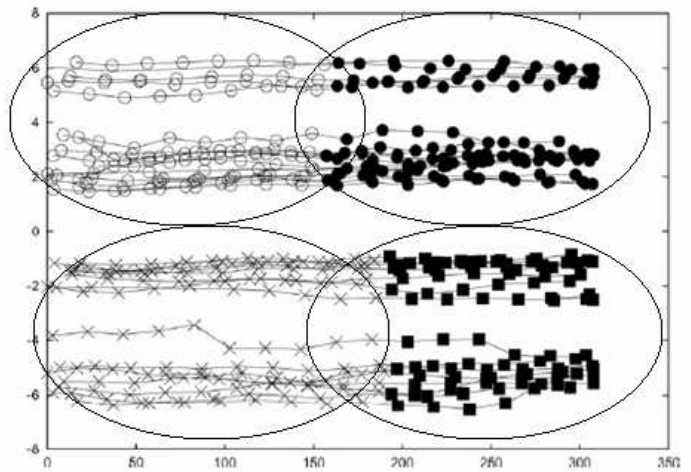
\includegraphics[scale=0.32]{gfx/ConstClust/GPS/Instancias} 
	\caption[Clustering of \acs{GPS} data with no constraints.]{Clustering of \acs{GPS} data with no constraints \cite{davidson2007survey,wagstaff2001constrained}.}\label{fig:figure15}
\end{figure}

\subsection{Recent Applications}

The aforementioned applications are the most studied in the literature, although the reader may have the impression that constrained clustering is no longer used in real-world problems. To prevent that, we provide a list of more recent applications of constrained clustering to modern problems: advanced robotics navigation systems \cite{semnani2016constrained}, applied marketing \cite{seret2014new}, obstructive sleep apnea analysis \cite{mai2018evolutionary}, handwritten digits classification \cite{li2015scalable}, Internet traffic classification \cite{wang2014internet}, electoral district designing, \cite{brieden2017constrained}, semantically similar relations identification \cite{wang2015constrained}, cooperative team building \cite{yang2014team}, video face clustering \cite{zhou2014video}, image clustering \cite{habashi2017semi} and storage location assignment in warehouses \cite{yang2016constrained}, among others.

\section{Benefits of Using Constraints} \label{sec:ConstraintsBenefits}

Two main benefits are found in the use of constraints:

\begin{itemize}
	
	\item Increased accuracy in label prediction by generating constraints based on a subset of labeled instances.
	
	\item Obtention of clusters with adaptable geometry to each problem.
	
\end{itemize}

These two benefits are discussed below:

Given $X = \{x_1 \cdots x_n\}$, a large set of unlabeled instances, and $L = \{(x_{n+1}, l_{n+1}) \cdots (x_{n+|L|}, l_{n+|L|})\}$, a small set of labeled instances, it is common to choose two elements from $L$ (with replacement) and set an \acs{ML} constraint between them if they belong to the same class, or a \acs{CL} constraint otherwise. An appropriate way to evaluate the results provided by a clustering method is to measure the level of accuracy it achieves when predicting dataset $X$ labels. This normally requires the number of desired clusters to be equal to the number of known classes in $X$ ($k = k^*$). Methods such as the RandIndex \cite{rand1971objective} or its variants, which will be discussed later, are used to measure the degree of agreement between two given partitions (clusterings).

In \cite{wagstaff2000clustering}, where constraints are generated as described above, it is shown that accuracy is increased up to 20\% over classic methods when averaging results over different constraint sets.

\begin{observation}
	
	\textbf{Using constraints increases average accuracy.}
	The performance of a method in predicting labels increases when averaged using numerous different constraint sets \cite{davidson2007survey}.
	\label{ob:AccuracyIncrease}
	
\end{observation}

This rule, however, is not always true, as in datasets such as \textit{Tic-Tac-Toe Endgame}, no increase in correct predictions is achieved regardless of the number of constraints used. A possible explanation for these exceptions is that setting $k = k^*$ may not be appropriate in these cases.

The other benefit of using constraints is the possibility of obtaining clusters with the desired geometry, such as the example of \acs{GPS} data clustering, analyzed in the Section \ref{sec:GPSApp}.

\section{Problems of Using Constraints} \label{sec:ConstraintsProblems}

Although, as we have seen, incorporating constraints into clustering methods brings benefits in some applications, there are two main drawbacks that are discussed below, as well as possible solutions to them.

\subsection{The Feasibility Problem} \label{sec:FeasibilityProblem}

The introduction of constraints into clustering changes the problem it solves, which becomes: \textit{Find the best partition that satisfies all constraints}. This way, if constraints are not properly specified or if the extraction methods are inadequate, we can end up with contradictory constraints, which means that there is no partition that satisfies them all. For instance, there is no partition that satisfies the constraints $C_=(x_i,x_j)$ and $C_{\neq}(x_i,x_j)$, regardless of the value of $k$. The same happens for $k = 2$, and the constraints $C_{\neq}(x_i, x_j)$, $C_{\neq}(x_j, x_q)$ and $C_{\neq}(x_i, x_q)$. Definition \ref{def:FeasibilityProblem} formalizes the feasibility problem for non-hierarchical instance-level constrained clustering:

\begin{definition}
	
	\textbf{Feasibility problem for non-hierarchical instance-level constrained clustering:} Given a dataset $X$, a constraint set $CS$, and the bounds on the number of clusters $k_l \leq k \leq k_u$, does there exist a partition $C$ of $X$ with $k$ clusters such that all constraints in $CS$ are satisfied? \cite{davidson2005clustering,davidson2007survey}
	
	\label{def:FeasibilityProblem}
	
\end{definition}

 The theoretical complexity of a constrained clustering problem depends on the type of constraints combined in it. Table \ref{tab:CCComplexity} summarizes the expected complexity in each case. 

\begin{table}[!h]
	\centering
	%\setlength{\arrayrulewidth}{1mm}
	%\setlength{\tabcolsep}{7pt}
	%\renewcommand{\arraystretch}{1}
	%\resizebox{\textwidth}{!}{
	\begin{tabular}{ >{\centering\arraybackslash}m{3cm}  >{\centering\arraybackslash}m{3cm} }
		\hline
		\textbf{Constraints} & \textbf{Complexity} \\
		\hline
		$\delta$ & $\mathbf{P}$ \\
		$\epsilon$ & $\mathbf{P}$ \\
		\acs{ML} and $\delta$ & $\mathbf{P}$ \\
		\acs{ML} and $\epsilon$ & $\mathbf{NP}$-complete \\
		$\epsilon$ and $\delta$ & $\mathbf{P}$ \\
		\acs{CL} and other & $\mathbf{NP}$-complete \\
		\hline
		
	\end{tabular}%}
	\caption[Complexity of the constrained clustering problem.]{Complexity of the constrained clustering problem \cite{davidson2007survey}.}
\label{tab:CCComplexity}
\end{table}

As shown in Table \ref{tab:CCComplexity}, the use of \acs{CL} constraints increases the complexity level of constrained clustering to $\mathbf{NP}$-complete and therefore constrained clustering is intractable. Intuitively, it can be easily understood that if finding a single partition that satisfies the constraints is a complex problem, finding the best of them is even harder.

\begin{observation}
	
	\textbf{Knowing a feasible solution exists does not help us find it.} The consequences of this result for the complexity of constrained clustering imply that, even if there is a feasible partition, it will not be easy to find in terms of algorithmic complexity \cite{davidson2007survey}.
	\label{ob:FeasibleSolution}
	
\end{observation}

In \cite{wagstaff2002intelligent} and \cite{davidson2007hierarchical} is shown that, even if the number of clusters in the output partition is equal to the number of classes in the dataset ($k = k^*$), which guarantees that a feasible solution does exist, simple algorithms like \acf{COPKM} \cite{wagstaff2001constrained} may not converge due to the feasibility problem.

\subsection{The Constraint Set Utility Problem} \label{sec:UtilityProblem}

In constrained clustering it is assumed that constraints are a guide for an algorithm to find the desired data partition. So, it would be reasonable to think that the more additional information (constraints) we have available, the closer the result will be to the one we are looking for, as Observation \ref{ob:AccuracyIncrease} stated. However, and despite the stipulations of this observation, we find cases where, even generating the constraints without noise and according to the true labels, there are constraint sets that, far from improving the results, worsen them considerably \cite{davidson2006proceedings}. This seems to disagree with Observation \ref{ob:AccuracyIncrease}; however, let us remember that it refers to the average case, and not to particular cases.

\begin{observation}
	
	\textbf{Individual constraint sets can have adverse effects}. Some constraint sets generated on the same ground truth labels that evaluate the clusters can cause a loss of accuracy at predicting those very labels \cite{davidson2007survey}.
	
\end{observation}

\subsection{Solutions for the Feasibility Problem} \label{sec:FeasibilityProblemSolutions}

The feasibility problem can be tackled in several ways. The most immediate may be to keep the number of constraints low (in proportion to the number of total instances) to minimize the likelihood of inconsistencies. However, not being able to increase the number of constraints if the problem requires it is not the ideal scenario. Attention should be paid to analyzing when a problem becomes over-constrained, since, as studied in Section \ref{sec:ConstraintsProblems}, even when constraint generation is based on the ground truth, algorithms such as \acs{COPKM} are no longer effective (not even with random restarts) as the number of constraints to be satisfied increases.

The problem over-constraining phenomenon through the use of \acs{CL} constraints is intimately related to the graph coloring problem. It has been proven that constrained clustering with \acs{CL} is equivalent to the graph coloring problem \cite{davidson2006identifying}. Thus, we find that solving a problem with \acs{CL} constraints using algorithms such as \acs{COPKM} is, in practice, solving the graph coloring problem.

\begin{observation}
	
	\textbf{Constrained clustering with \acs{CL} is analogous to the graph coloring problem} \cite{davidson2007survey}.
	
\end{observation}

This result allows us to transfer many of the properties of the graph coloring problem to the constrained clustering problem. For example, Brook's theorem states that graph coloring is simple when the number of available colors ($k$ in our case) is greater than the maximum degree of the graph.

\begin{observation}
	
	\textbf{Brook's theorem applies to the constrained clustering.}
	If $ k > $ (Most \acs{CL} constraints on an instance), then there always exists a feasible partition \cite{davidson2007survey} \label{ob:BrooksTheorem}.
	
\end{observation}

With this, and although Observation \ref{ob:FeasibleSolution} indicates differently, when constrained clustering meets the condition seen in Observation \ref{ob:BrooksTheorem}, we can guarantee that a solution will always be found in polynomial time. To ensure Brook's condition, it is possible to build the constraint set so that no instance appears in more than $k$ \acs{CL} constraints \cite{davidson2006identifying}.

\subsection{Solutions for the Constraint Set Utility Problem}

The solution to this problem is simple: truly useful constraint sets must be identified. However, this involves applying some kind of metric to evaluate the compliance of a given set of constraints with this condition. To this end two measures are proposed: informativity and coherence.

The \textbf{informativity} measure refers to the amount of information present in the constraint set that an algorithm cannot determine for itself. For example, in Figure \ref{fig:Informativity}, an algorithm such as \acs{COPKM} would tend to group nearby instances and place those that are far away in separate clusters; however, constraints bias the solution space preventing this from happening. 

\begin{figure}[!h]
	\centering
	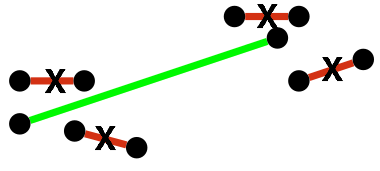
\includegraphics[scale=0.4]{gfx/ConstClust/Inform/Inform} 
	\caption[Informative constraint set.]{Informative constraint set \cite{davidson2007survey}.}\label{fig:Informativity}
\end{figure}


Informativity is estimated using the constraint set as a test set, so the ability of the algorithm to predict the constraints present in it is measured. Formally, given a set of constraints $CS$ and a constrained clustering algorithm $A$, we get the partition $C_A$ by applying the algorithm to the input dataset specifying an empty constraint set. We can compute the number of unsatisfied constraints in $C_A$ a in Equation \ref{eq:Informativity} \cite{davidson2007survey}.

\begin{equation}
I_A(CS) = \frac{1}{|CS|}\left[ \sum_{r \in CS} \text{unsat}(r, C_A) \right].
\label{eq:Informativity}
\end{equation}

\textbf{Coherence} measures the degree of agreement within the set of constraints itself with respect to a given metric. For instance, Figure \ref{fig:Coherence} shows two parallel and very close constraints of different type. It is in cases like this that the contradiction occurs, as the \acs{ML} constraints indicate that the distance between instances involved in them is small, while \acsp{CL} indicate the opposite.

\begin{figure}[!h]
	\centering
	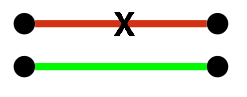
\includegraphics[scale=0.4]{gfx/ConstClust/Coherencia/Coher1}
	\caption[Non-coherent constraint set.]{Non-coherent constraint set \cite{davidson2007survey}.}\label{fig:Coherence}
\end{figure}

Then, the coherence measure is given by the degree of overlap that constraints produce by interpreting them as vectors in space and projecting them along one of the axes, as shown in Figure \ref{fig:CoherenceOverlap}.

\begin{figure}[!h]
	\centering
	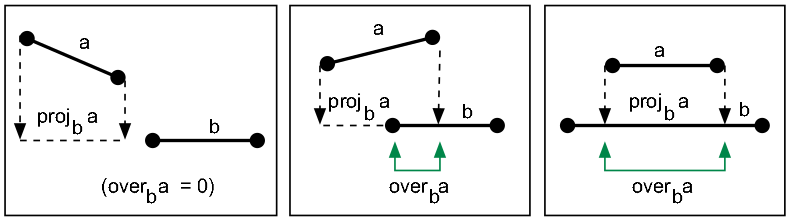
\includegraphics[scale=0.4]{gfx/ConstClust/Coherencia/Coher2}
	\caption[Coherence measure representation.]{Coherence measure representation \cite{davidson2007survey}.}\label{fig:CoherenceOverlap}
\end{figure}

\section{Summary}

Constrained clustering adds a new type of information to the original clustering problem, which is given in the form of specifications of belonging to the same or to different clusters on pairs of instances. Constraints, whether they are the pairwise \acf{ML} and \acf{CL} constraints, or the distance-based $\delta$ and $\epsilon$ constraints, are used to guide the clustering method being applied to a dataset in its search for a result partition that meets certain desired properties.

Clustering methods derived from this concept have proved to be advantageous in many areas; in addition to this, they suffer from some issues that can be tackled by carefully studying the constraints used to solve each individual problem.
